\documentclass[tikz, border=10pt]{standalone}
\usetikzlibrary{calc, angles, quotes}
\begin{document}
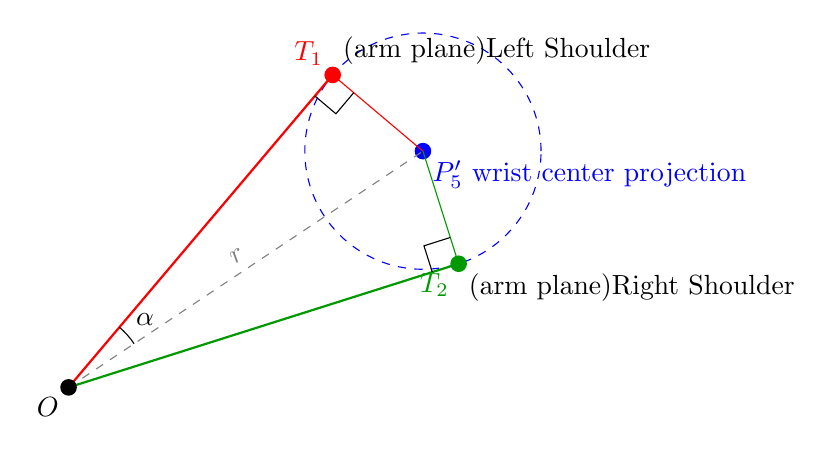
\begin{tikzpicture}[scale=1.5]
    % Points
    \coordinate (O) at (0,0);
    \coordinate (P) at (3,2);
    \def\r{1.0}

    % Distance from O to P, and tangent length
    \pgfmathsetmacro{\d}{sqrt(3*3 + 2*2)}
    \pgfmathsetmacro{\L}{sqrt(\d*\d - \r*\r)}
    \pgfmathsetmacro{\phi}{atan2(2, 3)}
    \pgfmathsetmacro{\alphaval}{asin(\r/\d)}

    % Tangent points by explicit trigonometry
    \coordinate (T1) at (\phi + \alphaval: \L);
    \coordinate (T2) at (\phi - \alphaval: \L);

    % Circle
    \draw[dashed, blue] (P) circle (\r);
    \fill[blue] (P) circle (2pt) node[below right] {\(P_5'\) wrist center projection};

    % Line from O to P
    \draw[gray, dashed] (O) -- (P) node[midway, sloped, above] {\(r\)};

    % Tangent lines
    \draw[red, thick] (O) -- (T1) node[above right, black] {(arm plane)Left Shoulder};
    \draw[green!60!black, thick] (O) -- (T2) node[below right, black] {(arm plane)Right Shoulder};

    % Radii to tangent points
    \draw[red, thin] (P) -- (T1);
    \draw[green!60!black, thin] (P) -- (T2);

    % Tangent points
    \fill[red] (T1) circle (2pt) node[above left] {\(T_1\)};
    \fill[green!60!black] (T2) circle (2pt) node[below left] {\(T_2\)};

    % Right angles
    \pic [draw, angle radius=0.35cm] {right angle = P--T1--O};
    \pic [draw, angle radius=0.35cm] {right angle = P--T2--O};

    % Angle alpha
    \pic [draw, "\(\alpha\)", angle radius=1.0cm, angle eccentricity=1.3]
         {angle = P--O--T1};

    % Origin
    \fill (O) circle (2pt) node[below left] {\(O\)};
\end{tikzpicture}
\end{document}